\chapter{Cálculo del \textit{Skeleton} Basado en la Distancia}
\label{ch:arcelli}

El tercer algoritmo implementado para esta tesis fue presentado por Arcelli et al. en \cite{arcelli2011distance}. Este algoritmo difiere en mayor medida de los dos anteriores porque utiliza la segunda definición del \textit{skeleton} presentada en el Capítulo \ref{ch:introduction}. En lugar de incendiar los objetos, el \textit{skeleton} es calculado a partir de los centros de las esferas maximales inscritas en el objeto.

El algoritmo cuya implementación se detalla en esta capítulo fue diseñado para calcular el \textit{skeleton} de imágenes 3D. Sin embargo, para adquirir familiaridad con las técnicas usadas, se comenzó por implementar el algoritmo para imágenes 2D basado en discos maximales que aparece en \cite{di1996skeletonization}. Este algoritmo 2D calcula el \textit{skeleton} siguiendo principios parecidos al algoritmo 3D de este capítulo, pero el operar exclusivamente sobre imágenes bidimensionales le concede una relativa sencillez. En los anexos se han dedicado unas palabras a esa versión.

\section{Fundamentos teóricos}

\subsection{Transformadas de distancia}

Una \textit{transformada de distancia} de una imagen es un etiquetado donde a cada píxel o vóxel de objeto se le asigna un número positivo que representa la distancia al píxel o vóxel de fondo más cercano. Los píxeles o vóxeles de fondo se etiquetan con el valor constante 0 \footnote{A veces los elementos de fondo son mapeados a otros valores, como por ejemplo a $\infty$, pero para los algoritmos de esta tesis se usa siempre 0.}. En otras palabras, la transformada de distancia es una matriz con las mismas dimensiones que su imagen correspondiente. Si un elemento de la imagen vale 0, en su mismo índice dentro de la transformada de distancia aparecerá un 0. Si un elemento de la imagen vale 1, en su mismo índice dentro de la transformada de distancia aparecerá un número positivo que indique la distancia entre ese elemento y el elemento con valor 0 más cercano. Estos valores positivos dependerán de cómo se mida la distancia entre dos elementos.

Fue necesario esbozar el concepto de transformada de distancia para explicar el algoritmo del Capítulo \ref{ch:siddiqi}. Dentro de ese algoritmo, el cálculo de la transformada de distancia euclidiana era el primer paso para el cálculo del \textit{skeleton}. Las operaciones subsecuentes eran de carácter global. En contraste, la métrica euclidiana no es adecuada para determinar localmente si un vóxel corresponde al centro de una esfera maximal. La transformada de distancia euclidiana busca ser exacta, por lo que no impone ninguna restricción que relacione los valores de vóxeles vecinos \cite{borgefors1991euclidean}. A pesar de esto, se han propuesto algunos algoritmos que la usan, como \cite{remy2003look}, basado en tablas de consulta con todos los valores posibles.

El algoritmo de este capítulo usa una transformada más amigable en el sentido anterior. Es parte de la familia de transformadas de distancia que se describe a continuación.

\subsection{La transformada de distancia <3,4,5>}

Una \textit{transformada de distancia con pesos} 3D es una transformada de distancia donde cada vóxel de objeto se etiqueta con el largo del 26-camino más corto que termina en un vóxel de fondo. Este tipo de transformada se calcula a partir de una 3-tupla $<p_c,p_a,p_v>$, donde $p_c$ es la distancia entre dos vóxeles que comparten una cara, $p_a$ es la distancia entre dos vóxeles que comparten una arista (pero no una cara) y $p_v$ es la distancia entre dos vóxeles que comparten un vértice (pero no una arista).

La idea básica de las transformadas de distancia con pesos es aproximar la transformada de distancia euclidiana, simplificando al mismo tiempo los cálculos. La transformada de distancia con pesos que interesa para este algoritmo es la $<3,4,5>$, cuyo error máximo con respecto a la euclidiana es del 12\% \cite{borgefors1996digital}.

\subsection{Centros de esferas maximales en la transformada de distancia <3,4,5>}
\label{ssec:hr_cmb}

La simplicidad de las transformadas de distancia con pesos permite encontrar máximos locales con facilidad. Dada una transformada de distancia con pesos $d$, puede decirse que un vóxel $v$ es el centro de una esfera maximal, CEM en adelante, comparando su etiqueta $d(v)$ con las de sus vecinos, tomando en cuenta los pesos según su relación de vecindad. En concreto, para la transformada de distancia $<3,4,5>$ un vóxel $v$ es CEM si sus vecinos cumplen las siguientes condiciones

\begin{enumerate}
\item $\forall n \in V_6(v), d(n) - d(v) < 3$,
\item $\forall n \in V_{18}(v), d(n) - d(v) < 4$ y
\item $\forall n \in V_{26}(v), d(n) - d(v) < 5$
\end{enumerate}

Estas condiciones buscan medir el grado de relevancia de la esfera maximal centrada en $v$. La relevancia de la esfera centrada en $v$ será mayor cuanto mayor sea el grado de solapamiento con las esferas centradas en sus vecinos (esto es, cada esfera de radio $d(n)$ centrada en $n$). Así, cuanto mayor sea alguna diferencia $d(n) - d(v)$, menor será la relevancia de $v$ como CEM.

La noción de relevancia permite refinar la detección de CEM. Así, se dice que un vóxel $v$ es un CEM \textit{altamente relevante} si cumple las condiciones

\begin{enumerate}
\item $\forall n \in V_6(v), d(n) - d(v) < 2$,
\item $\forall n \in V_{18}(v), d(n) - d(v) < 3$ y
\item $\forall n \in V_{26}(v), d(n) - d(v) < 4$
\end{enumerate}

\subsection{Capas en la transformada de distancia <3,4,5>}

Dado un vóxel $v$ y su correspondiente etiqueta $d(v)$, sus vecinos más alejados al borde del objeto pueden tener tres valores, $d(v) + p_c$, $d(v) + p_a$ y $d(v) + p_v$, dependiendo de su relación de vecindad. Siguiendo lo mostrado en \cite{svensson2002using}, esto permite dividir los vóxeles del objeto en subconjuntos llamados \textit{capas}, tal que los vóxeles $q$ de la capa $k$-ésima $C_k$ satisfacen
\DeclarePairedDelimiter{\ceil}{\lceil}{\rceil}
\begin{equation}
k = \ceil[\bigg]{\frac{d(q)}{p_c}}
\end{equation}
La Figura \ref{fig:arcelli_layers} ilustra este concepto. En ella, cada color en el corte axial del modelo representa una capa distinta.

\begin{figure}[H]\centering
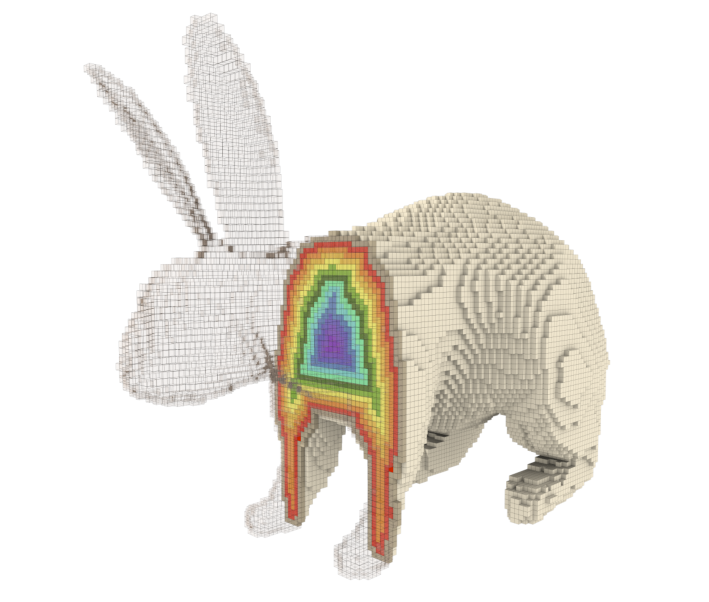
\includegraphics[width=0.7\linewidth]{images/arcelli_layers}
\caption{Capas en la transformada de distancia}
\label{fig:arcelli_layers}
\end{figure}

\subsection{Centros de esferas maximales esenciales}
\label{ssec:core_cmb}

Las capas pueden ser interpretadas como un frente que se propaga hacia el interior del objeto, en una versión aproximada de los principios del Capítulo \ref{ch:siddiqi}. Esta aproximación es imprecisa, pero puede ser usada como un segundo criterio de refinamiento para la detección de los CEM. En primer lugar, se dice que un vóxel $v$ de la capa $C_k$ es un centro de esfera maximal $esencial$ si cumple que

\begin{enumerate}
\item $v$ es un CEM altamente relevante y
\item $\forall n \in V_{26}(v), n \in C_k \rightarrow n$ es CEM
\end{enumerate}

Luego, si $v$ es un CEM esencial según el criterio anterior, todos los CEM altamente relevantes en $V_{26}(v)$ son también marcados como CEM esenciales.

Los CEM esenciales representan el verdadero punto de partida para este algoritmo. Los vóxeles marcados como CEM esenciales se consideran parte del \textit{skeleton} desde su detección. El resto del algoritmo consiste fundamentalmente de criterios para decidir cuándo eliminar a los demás vóxeles, con el fin de construir una \textit{skeleton} anclado en los CEM esenciales.

\section{Visión general del algoritmo}

\begin{algorithm}[H]
\caption{Skeletonización basada en distancia}
\label{alg:ddskel}
\begin{algorithmic}[1]
\Function{SkeletonizacionBasadaEnDistancia}{$I$, $\theta_1$, $\theta_2$}
	\State $td \gets TD345(I)$
    \State $cem \gets ExtraerCEM(td)$
    \State $anclas \gets Filtrar(cem)$
    \State $pss\_casi\_delgado \gets ErosionarYConectar(anclas)$
    \State $pss\_delgado \gets Adelgazar(pss\_casi\_delgado)$
    \State $pss \gets Podar(pss\_delgado, \theta_1, \theta_2)$ \label{ddprune1}
    \State $vc \gets ClasificarVoxeles(pss)$
    \State $tdd \gets TD345Delimitada(pss, vc)$
    \State $cem\_pss \gets ExtraerCEM(pss, tdd)$
    \State $anclas\_pss \gets Filtrar(cem\_pss)$
    \State $skeleton\_casi\_delgado \gets Erosionar(PSS, anclas\_pss)$
    \State $skeleton \gets Adelgazar(skeleton\_casi\_delgado)$
    \State $skeleton \gets Podar(skeleton, \theta_1, \theta_2)$ \label{ddprune2}
    \State \Return $skeleton$
\EndFunction
\end{algorithmic}
\end{algorithm}

En el pseudocódigo se observa que solamente los primeros pasos de este algoritmo corresponden a la detección de los CEM esenciales en la imagen de entrada. En la siguiente sección se detallan cada uno de los demás procedimientos. En resumen, tras detectar los CEM esenciales se sigue con un procesamiento que consiste en la erosión, adelgazamiento y poda de la imagen, conservando los CEM esenciales. Esto resulta en un \textit{skeleton} de superficie de la imagen. Luego, se detectan los CEM del \textit{skeleton} de superficie, y el procesamiento se vuelve a aplicar de manera similar.

\section{Descripción detallada de la implementación}

\subsection{Parámetros}

\begin{algorithm}[H]
\addtocounter{algorithm}{-1}
\caption{Parte 1}
\begin{algorithmic}[1]
\Function{SkeletonizacionBasadaEnDistancia}{$I$, $\theta_1$, $\theta_2$}
\algstore{bkbreak}
\end{algorithmic}
\end{algorithm}

Además de la imagen de entrada $I$, este algoritmo admite los parámetros numéricos $\theta_{1}$ y $\theta_{2}$, que permiten calibrar el nivel de detalle del \textit{skeleton}. Estos parámetros aparecen usados en las líneas \ref{ddprune1} y \ref{ddprune2} del pseudocódigo. Se trata de umbrales que determinan la eliminación de vóxeles de término. Su significado se detalla en la Sección \ref{ssec:prune1}.

\subsection{Cálculo de la transformada de distancia <3,4,5>}

\begin{algorithm}[H]
\caption{Parte 2}
\begin{algorithmic}[1]
\algrestore{bkbreak}
\State $TD \gets TD345(I)$
\algstore{bkbreak}
\end{algorithmic}
\end{algorithm}

Para calcular la transformada $<3,4,5>$ se implementó el algoritmo descrito en \cite{borgefors1996digital}. Este algoritmo permite calcular cualquier transformada de distancia con pesos en tiempo lineal respecto al número de vóxeles de la imagen. La imagen es recorrida dos veces, propagando los costos mínimos desde esquinas opuestas en cada pasada. El siguiente pseudocódigo describe este algoritmo.

\begin{algorithm}[H]
\caption{Cálculo de la transformada de distancia $<3,4,5>$}
\label{alg:ddskel}
\begin{algorithmic}[1]
\Function{TD345}{$I$}
	\State $d \gets Ceros(I)$
	\For{$i \gets 1, Dimension(I, 1)$} \Comment{Recorrido hacia adelante}
	\For{$j \gets 1, Dimension(I, 2)$}
	\For{$k \gets 1, Dimension(I, 3)$}
    	\If{$I_{i,j,k} = 1$}
        	\State $d_{i,j,k} \gets \min\limits_{(p,q,r) \in V_F}{d_{p,q,r} + p_n}$
        \EndIf
    \EndFor
    \EndFor
    \EndFor
	\For{$i \gets Dimension(I, 1), 1$} \Comment{Recorrido hacia atrás}
	\For{$j \gets Dimension(I, 2), 1$}
	\For{$k \gets Dimension(I, 3), 1$}
    	\If{$I_{i,j,k} = 1$}
        	\State $d_{i,j,k} \gets \min\limits_{(p,q,r) \in V_B}{d_{p,q,r} + p_n}$
        \EndIf
    \EndFor
    \EndFor
    \EndFor
    \State $ReemplazarValoresEquivalentes(d)$
    \State \Return $d$
\EndFunction
\end{algorithmic}
\end{algorithm}

El primer recorrido parte desde la esquina donde comienzan los índices en la implementación. Para cada vóxel de objeto $v$, $V_F(v)$ es el subconjunto ya recorrido de $V_{26}(v)$. $td(v)$ se calcula como el mínimo de tomar los valores de $td$ para ese conjunto y sumarles el peso $d_n$ correspondiente a la distancia local; por ejemplo, hay que sumar 5 a los vecinos que compartan solo un vértice con $v$. El segundo recorrido se efectúa en orden inverso. La única diferencia con el primer recorrido es que $V_B(v)$ contiene además el valor calculado para $v$ en el primer recorrido. Es decir, teniendo el largo del camino hacia el fondo encontrado en el primer recorrido, el segundo recorrido verifica si existe un camino más corto en alguna dirección no revisada.

Por último, la función $ReemplazarValoresEquivalentes()$ del final del algoritmo simplemente sustituye todos los valores 3 de la transformada por el valor 1. Este reemplazo permite la identificación correcta de máximos locales cercanos a los bordes \cite{arcelli1988finding}.

\subsection{Extracción de CEM}

\begin{algorithm}[H]
\caption{Parte 3}
\begin{algorithmic}[1]
\algrestore{bkbreak}
\State $cem \gets ExtraerCEM(I)$
\algstore{bkbreak}
\end{algorithmic}
\end{algorithm}

En este punto simplemente se etiqueta cada vóxel que cumple las condiciones para ser un CEM altamente relevante, de acuerdo a lo señalado en la Sección \ref{ssec:hr_cmb}. Como el criterio es local, la imagen debe ser recorrida una sola vez.

\subsection{Obtención de vóxeles de anclaje para el \textit{skeleton}}

\begin{algorithm}[H]
\caption{Parte 4}
\begin{algorithmic}[1]
\algrestore{bkbreak}
\State $anclas \gets Filtrar(CBM)$
\algstore{bkbreak}
\end{algorithmic}
\end{algorithm}

El principio básico detrás de este algoritmo es que el \textit{skeleton} se construye conectando los vóxeles de anclaje. En principio, los \textit{vóxeles de anclaje} son los CEM esenciales.

De entre los demás vóxeles se marcan también como vóxeles de anclaje aquellos que sean CEM altamente relevantes y además presenten una alta \textit{convexidad local}. La convexidad local de un vóxel $v$, denotada $T(v)$, se calcula como el número de 26-vecinos de $v$ con un valor de distancia mayor al de $v$ en la transformada de distancia. Entonces, los vóxeles $v$ que sean CEM altamente relevantes y para los cuales además $T(v)$ sea mayor a un umbral $\tau$ son marcados como vóxeles de anclaje. De acuerdo al artículo, un buen valor para $\tau$ es 7.

Se marcan además como vóxeles de anclaje los CEM altamente relevantes que pertenezcan a una componente 26-conexa de CEM que contenga al menos un CEM esencial. Este segundo criterio busca recalcar la importancia que se le da a las CEM esenciales.

\subsection{Obtención del PSS casi delgado}

\begin{algorithm}[H]
\caption{Parte 5}
\begin{algorithmic}[1]
\algrestore{bkbreak}
\State $pss\_casi\_delgado \gets ErosionarYConectar(anclas)$
\algstore{bkbreak}
\end{algorithmic}
\end{algorithm}

En el artículo de este algoritmo se explica cómo pequeños cambios en la implementación permitirían obtener un \textit{skeleton} de superficie competente. Sin embargo, para obtener el \textit{skeleton} curvilíneo es suficiente calcular primero lo que los autores llaman el \textit{pseudo-skeleton de superficie} (PSS), que se obtiene como resultado de las líneas 5 a la 7 del pseudocódigo. Se trata de un \textit{skeleton} de superficie simplificado, donde muchos vóxeles son eliminados de antemano porque no pertenecerán al \textit{skeleton} curvilíneo final.

El primer paso para obtener el PSS es idéntico al último paso del algoritmo del Capítulo \ref{ch:siddiqi}, salvo por el criterio de eliminación. Al igual que en el algoritmo de ese capítulo, los vóxeles de objeto son recorridos desde menor a mayor valor distancia. En este algoritmo un vóxel simple es candidato a eliminación si es que no fue marcado como vóxel de anclaje. Los vóxeles de anclaje son marcados como parte del PSS.

No obstante, simplemente quedarse con los vóxeles de anclaje no asegura que esta erosión produzca un resultado perceptualmente satisfactorio. La erosión producirá un PSS conectado, pero no hay garantía de que las conexiones entre los vóxeles de anclaje preserven alguna clase de simetría. Para remediar esto, cada vez que en el proceso de erosión se encuentra un vóxel de anclaje $v$, se marcan inmediatamente también como parte del PSS los vecinos más apropiados para conectar $v$ con el interior del objeto. El criterio para seleccionar estos vecinos consiste en buscar el o los vóxeles $n \in V_{26}(v)$ tales que $d(n) > d(v)$ y además maximicen la \textit{derivada direccional} en $V_{26}(v)$, definida como

\begin{equation}
\mathcal{D}_{(v,n)} = \frac{d(n) - d(v)}{p_n},
\end{equation}

\noindent
donde $p_n$ es el peso correspondiente a la relación de vecindad entre $n$ y $v$. Los vóxeles marcados según este criterio se denominan \textit{vóxeles de enlace}. Hasta el final del proceso de erosión se consideran equivalentes a los vóxeles de anclaje.

Por claridad es conveniente recalcar lo anterior. Cuando el proceso de erosión pasa de examinar el valor de distancia $m$ al valor $m + 1$, el criterio de la derivada direccional debe usarse para encontrar nuevos vóxeles de enlace que conecten hacia el interior del objeto tanto vóxeles de anclaje como de enlace, sean o no estos últimos vóxeles de anclaje al mismo tiempo.

El \textit{PSS casi delgado} se obtiene luego de procesar todos los valores para la distancia presentes en la transformada. Es ``casi delgado'' porque la inclusión de vóxeles de enlace puede originar regiones levemente gruesas.

\subsection{Adelgazamiento del PSS}

\begin{algorithm}[H]
\caption{Parte 6}
\begin{algorithmic}[1]
\algrestore{bkbreak}
\State $pss_delgado \gets Adelgazar(pss_casi_delgado)$
\algstore{bkbreak}
\end{algorithmic}
\end{algorithm}

El PSS casi delgado es erosionado usando máscaras, operando de manera similar al algoritmo del Capítulo \ref{ch:palagyi}. En este caso se usan las dos máscaras de la Figura \ref{fig:arcelli_directional_masks} para reducir las superficies de dos vóxeles de ancho.

\begin{figure}[H]\centering
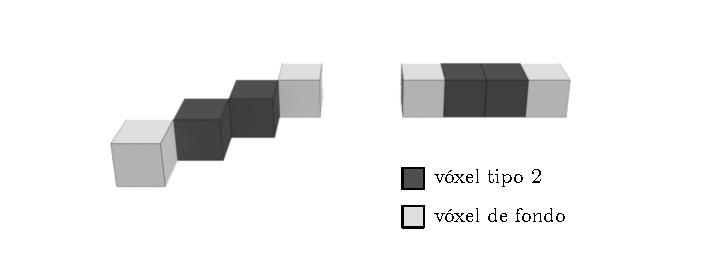
\includegraphics[width=0.8\linewidth]{images/arcelli_directional_masks}
\caption{Máscaras usadas para adelgazar el PSS}
\label{fig:arcelli_directional_masks}
\end{figure}

Los \textit{vóxeles tipo 2} son los vóxeles que satisfacen la segunda condición para la simplicidad señalada en la Sección \ref{ssec:3Dsimplicity}.

\subsection{Poda del PSS} \label{ssec:prune1}

\begin{algorithm}[H]
\caption{Parte 7}
\begin{algorithmic}[1]
\algrestore{bkbreak}
\State $PSS \gets Podar(PSSDelgado, \theta_1, \theta_2)$ \label{ddprune1}
\algstore{bkbreak}
\end{algorithmic}
\end{algorithm}

\subsection{Clasificación de vóxeles del PSS}

\begin{algorithm}[H]
\caption{Parte 8}
\begin{algorithmic}[1]
\algrestore{bkbreak}
\State $VC \gets ClasificarVoxeles(PSS)$
\algstore{bkbreak}
\end{algorithmic}
\end{algorithm}

\subsection{Cálculo de la transformada de distancia <3,4,5> del PSS}

\begin{algorithm}[H]
\caption{Parte 9}
\begin{algorithmic}[1]
\algrestore{bkbreak}
\State $TDD \gets TD345Delimitada(PSS, VC)$
\algstore{bkbreak}
\end{algorithmic}
\end{algorithm}


\subsection{Final}

\begin{algorithm}[H]
\caption{Parte 10}
\begin{algorithmic}[1]
\algrestore{bkbreak}
    \State $CBMPSS \gets ExtraerCBM(PSS, TDD)$
    \State $anclasPSS \gets Filtrar(CBMPSS)$
    \State $skeletonCasiDelgado \gets Erosionar(PSS, anclasPSS)$
    \State $skeleton \gets Adelgazar(skeletonCasiDelgado)$
    \State $skeleton \gets Podar(skeleton, \theta_1, \theta_2)$ \label{ddprune2}
    \State \Return $skeleton$
\EndFunction
\end{algorithmic}
\end{algorithm}

\section{Resultados}

\begin{figure}[ht]\centering5
\includegraphics[width=1\linewidth]{images/arcelli-3-25_test_models}
\caption{Resultados del algoritmo de Arcelli et al. para las imágenes de prueba, con $\theta_1 = 3$ y $\theta_2 = 0.25$}
\label{fig:arcelli-3-25_test_models}
\end{figure}

\begin{figure}[ht]\centering
\includegraphics[width=1\linewidth]{images/arcelli-7-25_test_models}
\caption{Resultados del algoritmo de Arcelli et al. para las imágenes de prueba, con $\theta_1 = 7$ y $\theta_2 = 0.25$}
\label{fig:arcelli-7-25_test_models}
\end{figure}